\sh{Overall Structure}
The proposed NoC architecture in Fig.~\ref{fig:System_Architecture} is designed to support three distinct Quality-of-Service (QoS) schemes in order to satisfy the heterogeneous communication requirements of different AXI4 masters and slaves:

\begin{figure}[htbp]
    \centering
    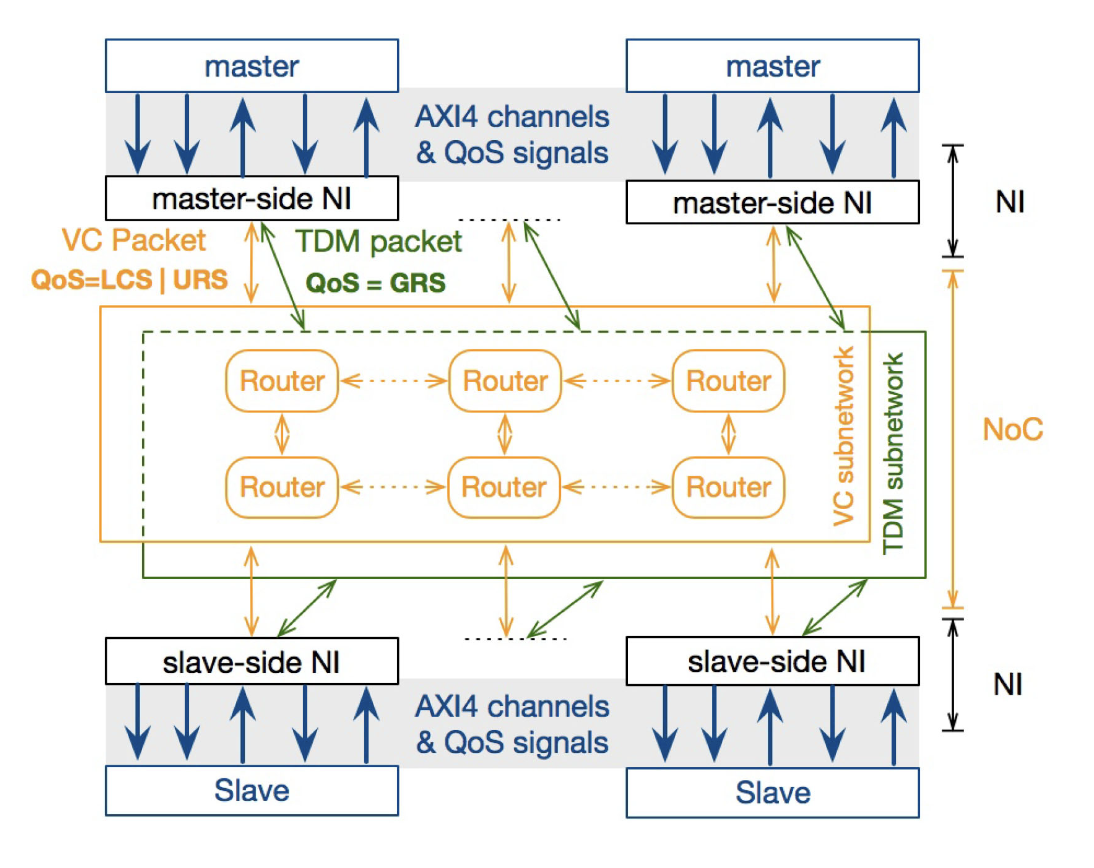
\includegraphics[width=0.95\textwidth]{img/System Architecture.png}
    \caption{System architecture}
    \label{fig:System_Architecture}
\end{figure}

\begin{itemize}
    \item \textbf{Latency-Critical Service (LCS):}\label{LCS} A low-latency forwarding service designed for bursty but non-streaming message transmissions. It provides fast delivery but does not guarantee bandwidth. Typical use cases include CPU-like masters that require short response times.
    \item \textbf{Guaranteed-Rate Service (GRS):}\label{GRS} A streaming service that ensures guaranteed bandwidth for large-volume data flows. It tolerates moderate latency but requires sustained throughput, as in GPU-like masters or other bandwidth-demanding accelerators.
    \item \textbf{Unspecified-Rate Service (URS):}\label{URS} A best-effort service that relies on currently available resources. It provides neither guaranteed bandwidth nor low latency, but aims at fairness among flows. URS is suitable for I/O interfaces such as SATA or USB.
\end{itemize}

To accommodate these QoS requirements, the system architecture is divided into three main components: (i) AXI4-based master/slave nodes, (ii) network interfaces (NIs) that perform protocol message conversion and QoS mapping, and (iii) the NoC fabric itself, which consists of two subnetworks: a VC-based subnetwork for LCS and URS traffic, and a TDM-based subnetwork for GRS traffic. 
This separation enables the NoC to meet diverse application needs without compromising performance or protocol compliance.


\sh{Message Format Conversion}
Two approaches can be used for message format conversion in AXI4-based NoCs. The first is a direct mapping, where each of the five AXI4 channels is converted into a separate packet format. In this case, the NoC must provide five dedicated paths in both subnetworks, one for each AXI4 channel. Although this preserves the semantics of AXI4, it couples the NoC tightly to the protocol, reduces design flexibility, and leads to poor resource utilization due to missing resource sharing. 
The second approach consolidates AXI4 transactions into four unified packet types: \textit{read request}, \textit{read response}, \textit{write request}, and \textit{write response}. These packets share the same NoC resources and are annotated with a QoS identifier (LCS, GRS, or URS), which determines whether they are routed through the VC or TDM subnetwork. This design choice decouples the NoC from the specifics of the AXI4 protocol, improves resource utilization, and enables compatibility with a wide range of interconnect architectures (e.g., buses or NoCs).
For these reasons, the authors adopt the second approach as the foundation of their high-performance and flexible AXI4-based NoC system. Based on this design, the network interface (NI) fulfills three core functionalities:
\begin{enumerate}
    \item \textbf{Dispatching:} The NI receives signals from the AXI4 channels and NoC subnetworks. 
    Transactions are dispatched either to the appropriate AXI4 channel (read/write) or to the correct NoC subnetwork (VC or TDM) according to their QoS identifier (LCS, GRS, URS).
    \item \textbf{Message format conversion:} The NI translates AXI4 transactions into NoC packets and vice versa, thereby decoupling the NoC fabric from protocol-specific details.
    \item \textbf{QoS inheritance:} On the slave side, response packets inherit the QoS class of their corresponding requests. 
    This ensures that QoS policies are consistently maintained across both request and response paths.
\end{enumerate}

Figure~\ref{fig:message_format} illustrates this process. AXI4 transactions from the five original channels (read address, read data, write address, write data, write response) are mapped into four packet types, labeled with QoS information, and forwarded to the appropriate subnetwork. On the return path, the QoS inheritance mechanism guarantees end-to-end service differentiation across the NoC.

\begin{figure}[htbp]
    \centering
    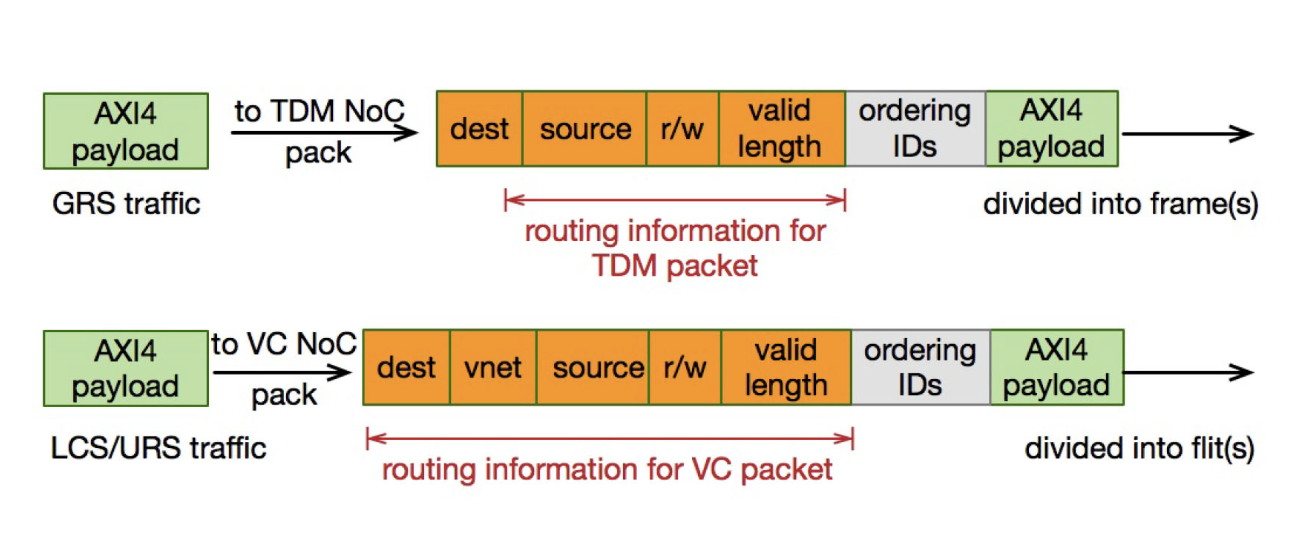
\includegraphics[width=0.95\textwidth]{img/Message format conversion.png}
    \caption{Message format conversion process in the NI}
    \label{fig:message_format}
\end{figure}


\sh{Master-Side and Slave-Side NI Architecture}
The master-side NI (see Figure~\ref{fig:master_NI}) converts AXI4 requests into NoC packets and assigns them to the appropriate subnetwork (VC or TDM) based on their QoS identifier (LCS, GRS, URS). It ensures that transactions are correctly encapsulated and routed to meet the QoS requirements of the originating master (e.g., CPU, GPU, I/O).
The slave-side NI (see Figure~\ref{fig:slave_NI}), on the other hand, unpacks NoC packets into AXI4 responses and delivers them to the slave devices. Since AXI4 response signals do not carry QoS identifiers, the slave-side NI applies a QoS inheritance mechanism, in which the response packet inherits the QoS class of its corresponding request. 
This mechanism guarantees that QoS policies are consistently enforced across both request and response paths, thereby maintaining end-to-end service differentiation in the NoC.

\begin{figure}
    \centering
    \begin{subfigure}[b]{0.48\textwidth}
        \centering
        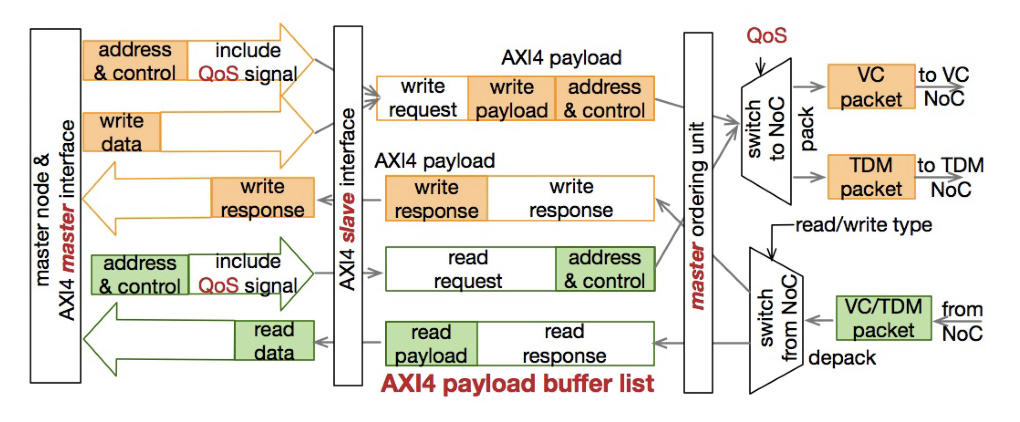
\includegraphics[width=\textwidth]{img/Master-Side_NI.png}
        \caption{Master-Side NI architecture}
        \label{fig:master_NI}
    \end{subfigure}
    \hfill
    \begin{subfigure}[b]{0.48\textwidth}
        \centering
        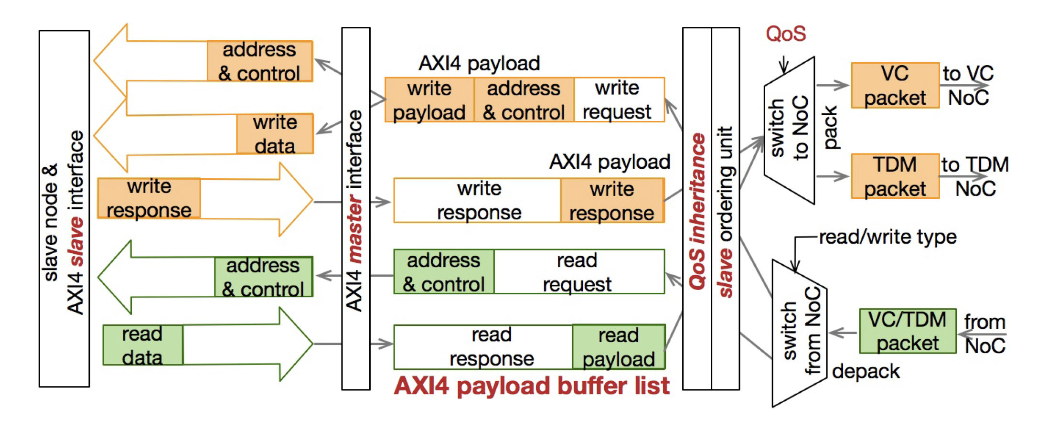
\includegraphics[width=\textwidth]{img/Slave-Side_NI.png}
        \caption{Slave-Side NI architecture}
        \label{fig:slave_NI}
    \end{subfigure}
    \caption{Slave- and Master-Side NI Architectures}
    \label{master_slave_ni}
\end{figure}


\sh{QoS Inheritance}
Because AXI4 response signals do not include QoS identifiers, the NI implements a QoS inheritance mechanism: the response packets automatically inherit the QoS information of their corresponding request packets. This ensures consistent QoS handling across request/response transactions.


\sh{Role of two Subnetworks (VC and TDM)}
To efficiently support heterogeneous QoS requirements, the NoC employs a dual-subnetwork structure:
\begin{itemize}
    \item The \textbf{VC subnetwork} (Virtual Channel) is used for LCS and URS packets. It provides low-latency transmission for critical traffic and fair, best-effort service for background traffic. Several flow control schemes are supported, ranging from strictly separated VCs for different QoS classes to shared VC approaches with priority arbitration.
    \item The \textbf{TDM subnetwork} (Time Division Multiplexing) is dedicated to GRS packets. By pre-allocating both paths and time slots, it guarantees bandwidth and ensures predictable latency for streaming traffic.
\end{itemize}
The separation into VC and TDM subnetworks prevents interference between different QoS services and allows resources to be allocated more effectively.


\sh{Flow Control Mechanisms in VC Subnetwork}
To manage virtual channel (VC) allocation and arbitration between latency-critical (LCS) and best-effort (URS) packets, four distinct flow control schemes are proposed. The \textit{Individual} scheme assigns dedicated VCs to each virtual network (VN), with LCS packets given higher priority. In the \textit{Individual\_Shared} scheme, all VCs are accessible to LCS packets, while URS packets are confined to a single fixed VC; LCS traffic continues to receive preferential treatment. The \textit{Total\_Shared} scheme allows both LCS and URS packets to share all VCs, although LCS packets are still prioritized during arbitration. Finally, the \textit{Standard} scheme treats all packets equally, with no prioritization across shared VCs. Among these, experimental evaluations indicate that the \textit{Individual\_Shared} scheme delivers the most favorable latency performance for LCS traffic.


\sh{Static Routing in TDM Subnetwork}  
The time-division multiplexing (TDM) subnetwork employs a static routing strategy based on a time-slot-driven routing table, which is constructed using a depth-first search algorithm. This approach enables the precomputation of routing paths, thereby eliminating runtime contention. Each router operates with synchronized time slots to deterministically forward packets, ensuring consistent and predictable delivery. The routing algorithm is designed to support round-trip communication while maintaining guaranteed bandwidth for streaming traffic. As a result, this static routing mechanism effectively minimizes latency and upholds the quality-of-service (QoS) requirements for guaranteed-rate service (GRS) flows.


\sh{Traffic Converter}
A key element of the NI is the \textit{Traffic Converter}, which dynamically balances the load between the two subnetworks: the VC (Virtual Channel) subnetwork and the TDM (Time-Division Multiplexing) subnetwork.
\begin{itemize}
    \item \textbf{VC to TDM Conversion:} When the VC subnetwork experiences congestion, selected latency-critical (LCS) packets are redirected to the TDM subnetwork. These packets are stored in a dedicated FIFO (GRS\_LCS FIFO) and scheduled with lower priority than native guaranteed-rate (GRS) traffic to preserve bandwidth guarantees.
    \item \textbf{TDM to VC Conversion:} If the TDM subnetwork is congested and VC is underutilized, GRS packets may be offloaded to the VC subnetwork. A controller estimates the queuing delay and determines whether rerouting will reduce latency. Converted packets are stored in the LCS\_GRS FIFO and fairly arbitrated with native LCS traffic.
\end{itemize}
This bidirectional conversion mechanism is implemented after the switch-to-NoC unit and before packetization, allowing real-time traffic adaptation. It improves overall utilization, reduces packet latency, and enhances throughput while maintaining QoS guarantees across traffic classes.

